\documentclass[11pt,a4paper]{article}

\usepackage[T1]{fontenc}
\usepackage[utf8]{inputenc}
\usepackage{newunicodechar}
\newunicodechar{ℝ}{\ensuremath{\mathbb{R}}}
\newunicodechar{∀}{\ensuremath{\forall}}
\newunicodechar{∃}{\ensuremath{\exists}}
\newunicodechar{≠}{\ensuremath{\neq}}
\newunicodechar{→}{\ensuremath{\to}}
\usepackage{mathptmx}
\usepackage[expansion=false]{microtype}
\usepackage[margin=2.6cm]{geometry}
\usepackage{amsmath,amssymb,amsthm,mathtools}
\usepackage{booktabs,tabularx,array}
\usepackage{enumitem}
\usepackage{xcolor}
\usepackage[most]{tcolorbox}
\usepackage{pgfplots}
\pgfplotsset{compat=1.16}
\usetikzlibrary{positioning,arrows.meta,fit,calc,backgrounds}
\usepackage[authoryear,round]{natbib}
\usepackage{xr-hyper}
\usepackage[colorlinks=true,linkcolor=blue!55!black,citecolor=blue!55!black,urlcolor=blue!55!black]{hyperref}

\setlist{itemsep=2pt,topsep=3pt,parsep=0pt}
\setlength{\emergencystretch}{3em}
\setlength{\parskip}{3pt}
\renewcommand{\arraystretch}{1.15}
\bibliographystyle{plainnat}

% ---------- theorem environments (one shared counter, numbered by section)
\theoremstyle{plain}
\newtheorem{theorem}{Theorem}[section]
\newtheorem{proposition}[theorem]{Proposition}
\newtheorem{lemma}[theorem]{Lemma}
\newtheorem{corollary}[theorem]{Corollary}
\theoremstyle{definition}
\newtheorem{definition}[theorem]{Definition}
\newtheorem{axiom}[theorem]{Axiom}
\newtheorem{property}[theorem]{Property}
\newtheorem{example}[theorem]{Example}
\theoremstyle{remark}
\newtheorem{remark}[theorem]{Remark}

% ---------- purpose line printed above every formal statement
\newcommand{\purpose}[1]{\par\smallskip\noindent{\small\upshape\leftskip=1.1em\rightskip=1.1em
  \textsc{Purpose.}\ #1\par}\vspace{-1pt}}

% ---------- notation
\newcommand{\R}{\mathbb R}
\newcommand{\E}{\mathbb E}
\newcommand{\LR}{\mathrm{LR}}
\newcommand{\Rext}{\widehat{\mathbb R}_\star}
\newcommand{\1}{\mathbf 1}
\newcommand{\TV}{\mathrm{TV}}
\newcommand{\ess}{\operatorname{ess\,sup}}
\newcommand{\eqd}{\overset{d}{=}}
\newcommand{\Hset}{\mathcal H}
\newcommand{\Xp}{\mathcal X}
\newcommand{\ax}[1]{\textup{(\textsf{#1})}}
\newcommand{\axCP}{\ax{CP}}
\newcommand{\axLI}{\ax{LI}}
\newcommand{\axCM}{\ax{CM}}
\newcommand{\axRC}{\ax{RC}}
\newcommand{\axRM}{\ax{RM}}
\newcommand{\bracket}[2]{[#1\!:\!#2]}

\newtcolorbox{keybox}[1][]{colback=blue!4!white,colframe=blue!45!black,
  boxrule=0.5pt,arc=2pt,left=6pt,right=6pt,top=4pt,bottom=4pt,breakable,#1}

\newcommand{\axP}{\ax{P}}
\newcommand{\cinf}[1]{c^{\infty}_{#1}}
\newcommand{\czero}[1]{c^{0}_{#1}}
\newcommand{\axN}{\ax{N}}
\newcommand{\axPe}{\textup{(\textsf{P}$_{\exists}$)}}
\newcommand{\axR}{\ax{R}}

% ---------- passages that record discussions between the author and the main assistant
\newenvironment{discussion}[1][]{\par\smallskip
  \begin{list}{}{\leftmargin=1.4em\rightmargin=1.4em\topsep=2pt\parsep=2pt}\item[]\small\itshape
  \textup{\textbf{$\diamond$\,Discussion}\if\relax\detokenize{#1}\relax\else\ \textmd{(#1)}\fi.}\ }
  {\end{list}\smallskip}

\externaldocument{main}

\renewcommand{\thesection}{S\arabic{section}}
\renewcommand{\thefigure}{S\arabic{figure}}
\renewcommand{\thetable}{S\arabic{table}}

\title{\textbf{Supplement to ``Reporting AI-Assisted Proofs in Mathematical Risk Management''}\\[4pt]
  \large Proofs, further results and records of the case study}
\author{Hirbod Assa}
\date{}

\begin{document}
\maketitle

\noindent This supplement contains the material of the case study that is not needed to follow the paper: the
proofs of the main results, a discussion of the role of the axioms, the version without law invariance, the
version for nonnegative losses, further consequences of the representation, a summary table of the literature, and
the timed record of the Lean check. References to sections, results and tables without the prefix S are to the
paper. The supplement is compiled together with the paper from the same source, which is available in the
repository \url{https://github.com/hirbod-assa/loss-ratio-lean}.

\tableofcontents

\section{Proofs of the main results}\label{sec:proofs}

Figure~\ref{fig:flow} shows the structure of the proof. Lemma~\ref{lem:R} derives the properties \axP, \axN{}
and \axCM{} from the axioms \axPe{} and \axR; Lemmas~\ref{lem:R}--\ref{lem:LI} are specific to loss ratios; Lemmas~\ref{lem:cashlip}--\ref{lem:rep} reprove the representation of comonotonic
additive functionals in the form needed here.

\begin{figure}[ht]
\centering\small
\fbox{\begin{minipage}{0.92\textwidth}\centering
\textbf{Lemma~\ref{lem:R}}: \axP, \axN, \axCM; additivity of the implied pair\ \ (\axPe, \axR)\\[2pt]
$\Updownarrow$\\[2pt]
\textbf{Lemma~\ref{lem:premium}} (implied premium): $\Pi$ from the price point; cash additive; $\Pi(c)=c$\ \ (\axP, \axN)\\[2pt]
$\Downarrow$\\[2pt]
\textbf{Lemma~\ref{lem:implied}} (implied risk measure): $\rho=\Pi\cdot\LR$ extends; Möbius cash lines\ \ (\axCM{} with sure losses)\\[2pt]
$\Downarrow$\\[2pt]
\textbf{Lemma~\ref{lem:comon}}: $\rho,\Pi$ comonotonic additive, also on the break-even set\ \ (\axCM)\\[2pt]
$\Downarrow$\\[2pt]
\textbf{Lemma~\ref{lem:LI}}: $\rho,\Pi$ law invariant\ \ (\axLI)\\[2pt]
$\Downarrow$\\[2pt]
\textbf{Lemma~\ref{lem:cashlip}}: homogeneity, Lipschitz\ \ (\axRC{} or \axRM, via Lemma~\ref{lem:offsets})\\[2pt]
$\Downarrow$\\[2pt]
\textbf{Lemma~\ref{lem:layer}}: layer formula; $h(p)=\rho(\1_A)$, $g(p)=\Pi(\1_A)$\ \ $\Rightarrow$\ \
\textbf{Lemma~\ref{lem:bv}}: bounded variation\ \ $\Rightarrow$\ \ \textbf{Lemma~\ref{lem:rep}}: $\rho=I_h$, $\Pi=I_g$
\end{minipage}}
\caption{Logical structure of the proof of Theorems~\ref{thm:A} and~\ref{thm:B}.}\label{fig:flow}
\end{figure}

\begin{lemma}[The derived properties]\label{lem:R}
Axioms \axPe{} and \axR{} hold if and only if \axP, \axN{} and \axCM{} hold. In that case, for every unpriced $W$
(that is, $\LR(W)\notin\R$) the quantity $r(W):=s\,(\LR(W+s)-1)$ does not depend on $s\ne0$, and the implied
premium and the implied risk measure satisfy $\Pi(X)=-\cinf X$ and $\rho(X)=\Pi(X)+r(X-\Pi(X))$ and are
comonotonic additive.
\end{lemma}

\begin{proof}
Assume \axPe{} and \axR. The quantities $\Pi,\rho,r$ below are used only in the proof; they appear in no axiom.

\emph{Step 0: \axP.} Let $\LR(Z)\notin\R$. The book $Z$ is comonotone with itself, so \axR{} applied to the pair
$(Z,Z)$ gives $\LR(Z+s)\in\R$ for every $s\ne0$. Hence a cash line has at most one non-finite point, and by \axPe{}
exactly one. So \axP{} holds; put $\Pi(X):=-\cinf X$, so that $\Pi(X+c)=\Pi(X)+c$ by \eqref{eq:pointscash}.

\emph{Step 1: \axN.} Let $p_0$ be the non-finite point of the cash line of $0$. Constants are comonotone, and
$\LR(p_0)\notin\R$, so \axR{} applied to $(p_0,p_0)$ gives $\LR(2p_0+u)\in\R$ for all $u\ne0$. If $p_0\ne0$, the choice
$u=-p_0$ gives $\LR(p_0)\in\R$, a contradiction; hence $p_0=0$ and $\LR(0)\notin\R$. Now apply \axR{} to $(0,0)$ with
$s=t=u$: $f(u):=u(\LR(u)-1)$ satisfies $f(u)=2f(u)$, so $f(u)=0$ and $\LR(u)=1$ for every $u\ne0$.

\emph{Step 2: the cash-line law.} Let $W$ be unpriced. The pair $(W,0)$ is comonotone and both books are unpriced,
so \eqref{eq:R} gives $u(\LR(W+u)-1)=s(\LR(W+s)-1)+t(\LR(t)-1)=s(\LR(W+s)-1)$ for all $s,t,u\ne0$, by Step 1. Hence
$r(W)$ does not depend on $s$. For any $X$ put $X_0:=X-\Pi(X)$, which is unpriced, and $\rho(X):=\Pi(X)+r(X_0)$. For
$c\ne-\Pi(X)$ write $X+c=X_0+s$ with $s=\Pi(X)+c\ne0$; then
\[
 \LR(X+c)=1+\frac{r(X_0)}{s}=\frac{\rho(X)+c}{\Pi(X)+c}.
\]
In particular $\rho=\Pi\cdot\LR$ on $D$, $\rho$ is cash additive, and $\rho(c)=\Pi(c)=c$.

\emph{Step 3: comonotonic additivity.} Let $X,Y$ be comonotone. Cash shifts preserve comonotonicity, so $X_0$ and
$Y_0$ are comonotone and unpriced. By \axR, $\LR(X_0+Y_0+u)\in\R$ for every $u\ne0$; by \axP{} the non-finite point of
the cash line of $X_0+Y_0$ is therefore $0$, so $\Pi(X_0+Y_0)=0$, that is, $\Pi(X+Y)=\Pi(X)+\Pi(Y)$. Consequently
$(X+Y)_0=X_0+Y_0$, and \eqref{eq:R} with $s=t=u$ gives $r(X_0+Y_0)=r(X_0)+r(Y_0)$; hence $\rho(X+Y)=\rho(X)+\rho(Y)$.
No premium is recovered from finite values, so the argument covers break-even books, pairs of which only one
breaks even, the case $\LR\equiv1$ on $D$, and pools whose premiums cancel. By Lemma~\ref{lem:comon}(b), which needs
only \axP{} and \axN, \axCM{} holds, and the implied risk measure of Definition~\ref{def:impliedrisk} is the
functional $\rho$ just constructed.

\emph{Converse.} Assume \axP, \axN, \axCM. Then \axPe{} is clear. By Proposition~\ref{prop:readings}(a) and
Lemma~\ref{lem:comon}(a), every cash line is $\LR(X+c)=(\rho(X)+c)/(\Pi(X)+c)$ and $\rho,\Pi$ are comonotonic
additive. Let $X,Y$ be comonotone and unpriced, so $\Pi(X)=\Pi(Y)=0$. For $s\ne0$, $\LR(X+s)=(\rho(X)+s)/s\in\R$ and
$s(\LR(X+s)-1)=\rho(X)$, and likewise for $Y$. Moreover $\Pi(X+Y)=0$, so $\LR(X+Y+u)\in\R$ for $u\ne0$ and
$u(\LR(X+Y+u)-1)=\rho(X+Y)=\rho(X)+\rho(Y)$, which is \eqref{eq:R}. \qedhere
\end{proof}

\begin{proof}[Proof of Proposition~\ref{prop:RPNCM}]
This is the first statement of Lemma~\ref{lem:R}. \qedhere
\end{proof}

\begin{lemma}[The cash offsets]\label{lem:offsets}
Assume \axPe{} and \axR, and let $X\in L^\infty$, $a\in\R$ and $W=X-a$. Then $\LR(W)\notin\R$ if and only if
$a=\Pi(X)$; and [$\LR(W)=0$, or $\LR(W)\notin\R$ and $\LR(W+1)=1$] if and only if $a=\rho(X)$. Consequently \axRC{}
holds if and only if $\Pi$ and $\rho$ are uniformly continuous, and \axRM{} holds if and only if $\Pi$ and $\rho$ are
monotone.
\end{lemma}

\begin{proof}
The first statement is the definition of the price point. For the second, $\Pi(W)=\Pi(X)-a$ and $\rho(W)=\rho(X)-a$.
If $\Pi(W)\ne0$, then $W$ is not unpriced and $\LR(W)=\rho(W)/\Pi(W)$, which vanishes exactly when $\rho(W)=0$. If
$\Pi(W)=0$, then $\LR(W)\notin\R$ and $\LR(W+1)=\rho(W)+1$ by Lemma~\ref{lem:R}, which equals $1$ exactly when
$\rho(W)=0$. In both cases the condition means $a=\rho(X)$. The axioms \axRC{} and \axRM{} therefore compare
$\Pi(X)$ with $\Pi(Y)$ in (i) and $\rho(X)$ with $\rho(Y)$ in (ii). \qedhere
\end{proof}

\begin{lemma}[Implied premium]\label{lem:premium}
Assume \axP. Then $\Pi(X+c)=\Pi(X)+c$ for all $X$ and $c$, and $D=\{\Pi\ne0\}$. If also \axN, then
$\Pi(c)=c$ for every constant $c$.
\end{lemma}

\begin{proof}
The cash line of $X+c$ is $d\mapsto\LR(X+c+d)$, the cash line of $X$ shifted by $c$; its price point is
therefore the price point of $X$ minus $c$, which is \eqref{eq:Picash}. $X\in D$ means that $0$ is not the
price point, i.e.\ $\Pi(X)\ne0$. Under \axN{} the cash line of $0$ takes the value $1$ at every $d\neq0$, so
its price point is $0$, $\Pi(0)=0$, and $\Pi(c)=c$. \qedhere
\end{proof}

\begin{lemma}[Implied risk measure]\label{lem:implied}
Assume \axP, \axN, \axCM. If $X\in D$ and $X+c\in D$, then $\rho(X+c)=\rho(X)+c$. Consequently
$\rho(X):=\rho(X+c)-c$, for any $c\ne-\Pi(X)$, defines a cash-additive functional on $L^\infty$ that agrees
with $\Pi\cdot\LR$ on $D$, satisfies $\rho(c)=c$, and
\begin{equation}\label{eq:mobius}
 \LR(X+c)=\frac{\rho(X)+c}{\Pi(X)+c}\qquad\text{for all }c\ne-\Pi(X).
\end{equation}
\end{lemma}

\begin{proof}
Let $X,X+c\in D$ with $c\ne0$. The constant $c$ lies in $D$ (by \axN), is comonotone with $X$, and
$\Pi(X)+\Pi(c)=\Pi(X+c)\ne0$ by Lemma~\ref{lem:premium}. So \axCM{} applies to the pair $(X,c)$ and gives
$\LR(X+c)=(\Pi(X)\LR(X)+c)/(\Pi(X)+c)$, i.e.\ $\rho(X+c)=\Pi(X+c)\LR(X+c)=\rho(X)+c$.

For arbitrary $X$, $X+c\in D$ exactly when $c\ne-\Pi(X)$. If $c,c'$ are two such values, then
$X+c'=(X+c)+(c'-c)$ with both $X+c$ and $X+c'$ in $D$, so $\rho(X+c')=\rho(X+c)+(c'-c)$; hence
$\rho(X+c)-c$ does not depend on $c$, and for $X\in D$ (take $c=0$) it equals $\Pi(X)\LR(X)$. Cash additivity
of the extension is immediate. For $c\neq-\Pi(X)$,
$\LR(X+c)=\rho(X+c)/\Pi(X+c)=(\rho(X)+c)/(\Pi(X)+c)$. Finally $\rho(c)=\Pi(c)\LR(c)=c$ for $c\ne0$, and
$\rho(0)=\rho(1)-1=0$. \qedhere
\end{proof}

\begin{proof}[Proof of Proposition~\ref{prop:readings}]
(a) is \eqref{eq:mobius}, and (b) restates it. For (c), $(c+\Pi(X))\LR(X+c)=\rho(X)+c\to\rho(X)-\Pi(X)$ as
$c\to-\Pi(X)$. For (d), the right-hand side of \eqref{eq:mobius} vanishes only at $c=-\rho(X)$, which differs
from the price point when $\rho(X)\ne\Pi(X)$; when $\rho(X)=\Pi(X)$ it equals $1$ for every $c\ne-\Pi(X)$.
Uniqueness of the extension is clear, since any cash-additive extension must satisfy (b). \qedhere
\end{proof}

\begin{lemma}[Comonotonic additivity]\label{lem:comon}
Assume \axP{} and \axN.
\begin{enumerate}[label=(\alph*),nosep]
\item If \axCM{} holds, then $\rho$ and $\Pi$ are comonotonic additive.
\item Conversely, if $\Pi$ is comonotonic additive and there is a comonotonic additive $\tilde\rho$ with
  $\tilde\rho=\Pi\cdot\LR$ on $D$, then \axCM{} holds and the implied risk measure equals $\tilde\rho$.
\end{enumerate}
\end{lemma}

\begin{proof}
(a) Let $X,Y$ be comonotone, $Z=X+Y$, $r=\rho(X)+\rho(Y)$ and $q=\Pi(X)+\Pi(Y)$. Fix $s\neq-q$ and choose
$u\notin\{-\Pi(X),\,s+\Pi(Y)\}$.
\begin{enumerate}[label=(\arabic*),nosep]
\item $X+u$ and $Y+s-u$ are comonotone, and by Lemma~\ref{lem:premium} their premiums $\Pi(X)+u$ and
  $\Pi(Y)+s-u$ are non-zero. So both lie in $D$, and their premiums sum to $q+s\neq0$.
\item Apply \axCM{} to this pair and use $\rho=\Pi\cdot\LR$ on $D$ with Lemma~\ref{lem:implied}:
  \[
  \LR(Z+s)=\frac{(\rho(X)+u)+(\rho(Y)+s-u)}{q+s}=\frac{r+s}{q+s}\in\R .
  \]
\item Thus the cash line of $Z$ is finite at every $s\neq-q$. By \axP{} it has exactly one non-finite
  point, so that point is $-q$, and $\Pi(Z)=q$.
\item For $s\ne-q$, Lemma~\ref{lem:implied} gives $\rho(Z)+s=\rho(Z+s)=\Pi(Z+s)\LR(Z+s)=r+s$, so $\rho(Z)=r$.
\end{enumerate}
The argument never asks whether $X$, $Y$ or $Z$ break even: \axP{} locates the price point even when the
cash line equals $1$ everywhere else.

(b) Let $X,Y\in D$ be comonotone with $q=\Pi(X)+\Pi(Y)\ne0$. Then $\Pi(X+Y)=q\ne0$, so $X+Y\in D$, and
$\LR(X+Y)=\tilde\rho(X+Y)/q=(\tilde\rho(X)+\tilde\rho(Y))/q=(\Pi(X)\LR(X)+\Pi(Y)\LR(Y))/q$. Both $\tilde\rho$ and
the implied risk measure are cash additive (the former by additivity with constants and $\tilde\rho(c)=\Pi(c)\LR(c)=c$)
and agree on $D$, hence everywhere. \qedhere
\end{proof}

\begin{lemma}[Law invariance of the implied pair]\label{lem:LI}
Assume \axP, \axN, \axCM{} and \axLI. Then $\rho$ and $\Pi$ are law invariant.
\end{lemma}

\begin{proof}
If $X\eqd Y$ then $X+c\eqd Y+c$ for every $c$, so by \axLI{} the cash lines of $X$ and $Y$ have the same finite
values and the same non-finite locations. Hence they have the same price point, $\Pi(X)=\Pi(Y)$, and by Proposition~\ref{prop:readings}(b) $\rho(X)=\rho(Y)$. \qedhere
\end{proof}

\begin{lemma}[Homogeneity and Lipschitz continuity]\label{lem:cashlip}
Assume \axP, \axN, \axCM, and let $F\in\{\rho,\Pi\}$. If \axRC{} or \axRM{} holds, $F$ is positively homogeneous
and Lipschitz; under \axRM{} it is $1$-Lipschitz.
\end{lemma}

\begin{proof}
By Lemma~\ref{lem:offsets}, $\rho$ and $\Pi$ are uniformly continuous under \axRC, and monotone under \axRM.
Since $X$ is comonotone with itself, $F(nX)=nF(X)$ by Lemma~\ref{lem:comon}, so $F(qX)=qF(X)$ for rational $q>0$.
\emph{Under \axRM:} $X\le Y+\|X-Y\|$ gives $F(X)\le F(Y)+\|X-Y\|$ by monotonicity and cash additivity, so $F$ is
$1$-Lipschitz, and homogeneity extends to real $\lambda>0$. \emph{Under \axRC:} continuity gives
$F(\lambda X)=\lambda F(X)$ for real $\lambda>0$. Choose $\delta>0$ with $|F(X')-F(Y')|\le1$ whenever
$\|X'-Y'\|\le\delta$, and apply it to $tX,tY$ with $t=\delta/\|X-Y\|$; this gives
$|F(X)-F(Y)|\le\|X-Y\|/\delta$. \qedhere
\end{proof}

\begin{lemma}[Layer formula]\label{lem:layer}
Assume \axP, \axN, \axCM, \axLI{} and \axRC{} (or \axRM). Define, for $P(A)=p$, $h(p):=\rho(\1_A)$ and
$g(p):=\Pi(\1_A)$. These are well defined by Lemma~\ref{lem:LI}, defined for every $p\in[0,1]$ because the
space is atomless, and $h(0)=g(0)=0$, $h(1)=g(1)=1$. For every chain $C_1\supset\dots\supset C_m$, $x_0\in\R$
and $a_i\ge0$,
\begin{equation}\label{eq:layer}
 \rho\Big(x_0+\sum_i a_i\1_{C_i}\Big)=x_0+\sum_i a_i\,h(P(C_i)),
\end{equation}
and likewise for $\Pi$ with $g$.
\end{lemma}

\begin{proof}
The partial sum $S_{j-1}=\sum_{i<j}a_i\1_{C_i}$ attains its maximum on $C_j$, so it is comonotone with
$\1_{C_j}$. Apply Lemma~\ref{lem:comon} and cash additivity successively, with
$\rho(a\1_C)=a\rho(\1_C)=a\,h(P(C))$ by Lemma~\ref{lem:cashlip}. The values at $0$ and $1$ come from
$\rho(0)=\Pi(0)=0$ and $\rho(1)=\Pi(1)=1$. \qedhere
\end{proof}

\begin{lemma}[Bounded variation]\label{lem:bv}
Under the assumptions of Lemma~\ref{lem:layer}, $h,g\in\Hset_1$. Under \axRM{} they are non-decreasing.
\end{lemma}

\begin{proof}
\emph{Under \axRM.} For $p\le q$ choose nested $A\subset B$ with $P(A)=p$, $P(B)=q$; then $\1_A\le\1_B$ gives
$h(p)\le h(q)$, and likewise for $g$.

\emph{Under \axRC.} Let $L$ be a Lipschitz constant of $\rho$. Take $0=p_0<\dots<p_n=1$ and a uniform random
variable $U$. Put $I_j=\{1-p_j<U\le1-p_{j-1}\}$ and $\delta_j=h(p_j)-h(p_{j-1})$. For $\sigma\in\{0,1\}^n$ let
$W=\sum_j2(n-j)\1_{I_j}$ and $Y_\sigma=W+\sum_j\sigma_j\1_{I_j}$. The values $2(n-j)+\sigma_j$ are strictly
decreasing in $j$, so $W$ and $Y_\sigma$ have the same upper sets $\{U>1-p_j\}$, of probability $p_j$. By
\eqref{eq:layer} and summation by parts, $\rho\big(\sum_jv_j\1_{I_j}\big)=\sum_jv_j\delta_j$ for every
non-increasing $v\ge0$. Hence $|\sum_j\sigma_j\delta_j|=|\rho(Y_\sigma)-\rho(W)|\le L\|Y_\sigma-W\|\le L$.
Choosing $\sigma_j=\1\{\delta_j>0\}$ and then $\sigma_j=\1\{\delta_j<0\}$ gives $\sum_j|\delta_j|\le2L$. \qedhere
\end{proof}

\begin{lemma}[Representation]\label{lem:rep}
Under the assumptions of Lemma~\ref{lem:layer}, $\rho=I_h$ and $\Pi=I_g$.
\end{lemma}

\begin{proof}
For a simple $X=x_0+\sum_ia_i\1_{C_i}$ with $a_i\ge0$ and $C_i=\{X\ge x_i\}$, a direct computation gives
$I_h(X)=x_0+\sum_ia_ih(P(C_i))=\rho(X)$. Simple positions are uniformly dense in $L^\infty$, and $\rho$ and
$I_h$ are both Lipschitz (Lemma~\ref{lem:cashlip} and $|I_h(X)-I_h(Y)|\le\TV(h)\|X-Y\|$), so $\rho=I_h$.
Likewise $\Pi=I_g$. \qedhere
\end{proof}

\begin{proof}[Proof of Theorems~\ref{thm:A} and~\ref{thm:B}]
\emph{(i)$\Rightarrow$(ii).} By Lemma~\ref{lem:R}, \axP, \axN{} and \axCM{} hold. Lemmas~\ref{lem:premium}--\ref{lem:rep} then give $\Pi=I_g$ and $\rho=I_h$ with
$h,g\in\Hset_1$, non-decreasing under \axRM. On $D=\{\Pi\ne0\}=\{I_g\ne0\}$, $\LR=\rho/\Pi=I_h/I_g$, and off $D$
the loss ratio is not finite. Under \ax{S}, at a book with $I_g(X)=0$ the label is $\star$ exactly when the
residue $\rho(X)=I_h(X)$ vanishes, which is the value of $\bracket{I_h(X)}{0}$.

\emph{(ii)$\Rightarrow$(i).} Let $\LR$ be as in (ii). Since $I_g(X+c)=I_g(X)+c$, the cash line of $X$ is non-finite
exactly at $c=-I_g(X)$, so \axP{} holds and $\Pi=I_g$. \axN{} holds because $I_h(c)=I_g(c)=c$. Next, $I_k$ is
comonotonic additive for $k\in\Hset$: for comonotone $X,Y$, any two upper sets $\{X\ge a\}$, $\{Y\ge b\}$ are almost
surely nested (otherwise comonotonicity fails on a $P\otimes P$-positive set); for simple comonotone $X,Y$ the
union of their upper sets is therefore a chain, giving $X=x_0+\sum a_i\1_{C_i}$, $Y=y_0+\sum b_i\1_{C_i}$ with
$a_i,b_i\ge0$, and additivity follows from the layer computation; for general $X,Y$ approximate by the comonotone
simple pairs $\lfloor nX\rfloor/n$, $\lfloor nY\rfloor/n$ and use the Lipschitz bound. Lemma~\ref{lem:comon}(b) with
$\tilde\rho=I_h$ gives \axCM{} and $\rho=I_h$. Hence \axPe{} and \axR{} hold by Lemma~\ref{lem:R}. \axLI{} holds because $I_k$ depends on $X$ only through
$x\mapsto P(X>x)$. By Lemma~\ref{lem:offsets} the two sure amounts in \axRC{} and \axRM{} are $I_g(X)$ and $I_h(X)$, so
\axRC{} holds because $I_h,I_g$ are Lipschitz, and \axRM{} when $h,g$ are non-decreasing. \qedhere
\end{proof}

\begin{proof}[Proof of Propositions~\ref{prop:unique} and~\ref{prop:derived}]
$g(p)=\Pi(\1_A)$ is minus the price point of $\1_A$, and $h(p)=\rho(\1_A)$ is given by
Proposition~\ref{prop:readings}(b); both are determined by $\LR$, including when $h=g$. The identities for $D$ and
$N$ follow from $\Pi=I_g$, $\rho=I_h$. Monotonicity of $\rho$ is equivalent to monotonicity of $h$ because $I_h$ is
monotone if and only if $h$ is non-decreasing. Proposition~\ref{prop:derived} collects
Lemmas~\ref{lem:premium}--\ref{lem:comon} and~\ref{lem:cashlip}, the Lipschitz bound for $I_k$, and
$\LR(\lambda X)=\lambda\rho(X)/(\lambda\Pi(X))=\LR(X)$ on $D$ (and $\lambda D=D$). \qedhere
\end{proof}

\section{On the role of the axioms}\label{sec:triviality}

\subsection{Structure of the result}

The proof of Theorem~\ref{thm:A} has three steps.

\begin{enumerate}[label=(\Alph*),leftmargin=*,itemsep=2pt]
\item \emph{Implied pair.} Axioms \axPe{} and \axR{} give \axP, \axN{} and \axCM{} (Lemma~\ref{lem:R}). Property \axP{}
  defines $\Pi$; \axR{} with a sure loss, equivalently \axN{} and \axCM{} applied with sure losses, defines $\rho$ and
  gives the Möbius form of the cash lines (Lemmas~\ref{lem:R}, \ref{lem:premium} and~\ref{lem:implied}).
\item \emph{Transfer.} Given \axP{} and \axN, \axCM{} holds if and only if $\rho$ and $\Pi$ are comonotonic
  additive (Lemma~\ref{lem:comon}), and \axLI{} passes from $\LR$ to $\rho$ and $\Pi$ (Lemma~\ref{lem:LI}).
\item \emph{Representation.} A law-invariant, comonotonic additive, uniformly continuous functional on an
  atomless $L^\infty$ is a signed Choquet integral \citep[Thm.~1]{www2020}; under monotonicity it is a
  distortion premium \citep{schmeidler1986,wyp1997}.
\end{enumerate}

Step (C) is classical; we reprove it in Section~\ref{sec:proofs} to keep the constants explicit and to show that
no continuity is needed in the monotone case. Steps (A) and (B) are specific to loss ratios. Together, axioms
\axPe{} and \axR{} state that $\LR$ is the ratio of a pair of comonotonic additive functionals that coincide
with the identity on constants, and that this pair can be read off $\LR$.

\subsection{Assumed and derived properties}

Table~\ref{tab:derived} lists the properties of the representation and their source. Axiom \axPe{} is ordinal,
and \axLI, \axRC, \axRM{} select the class of representing functions. The cardinal content of the axioms lies in
\axR, which contains the normalization \axN{} and the pooling property \axCM; given \axP{} and \axN, \axCM{} is equivalent to
comonotonic additivity of the implied premium and risk measure, which is the axiom that produces Choquet
representations in \citet{yaari1987}, \citet{schmeidler1986} and \citet{wyp1997}. The Choquet form of the numerator
and the denominator is therefore a consequence of comonotonic additivity, as in the single-functional case.

\begin{table}[ht]
\centering\small
\begin{tabularx}{\textwidth}{@{}>{\raggedright\arraybackslash}p{4.8cm}>{\raggedright\arraybackslash}X>{\raggedright\arraybackslash}p{2.0cm}@{}}
\toprule
\textbf{Property} & \textbf{Source} & \textbf{Status}\\
\midrule
unique price point (\axP); $\Pi$ cash additive & \axPe{} and \axR{} (Lemma~\ref{lem:R}) & derived\\
$\LR(c)=1$ (\axN); $\Pi(c)=c$, $\rho(c)=c$ & \axR{} (Lemma~\ref{lem:R}) & derived\\
$\rho$ defined on $L^\infty$; Möbius cash lines & \axR{} with a sure loss (Lemma~\ref{lem:R}) & derived\\
$\rho,\Pi$ comonotonic additive; \axCM & \axR{} (Lemmas~\ref{lem:R} and~\ref{lem:comon}) & equivalent\\
$\rho,\Pi$ law invariant & \axLI{} (Lemma~\ref{lem:LI}) & assumed\\
$\rho,\Pi$ continuous or monotone & \axRC, \axRM{} & assumed\\
$h,g$ of bounded variation & Lemma~\ref{lem:bv} & derived\\
$\rho=I_h$, $\Pi=I_g$ & Lemmas~\ref{lem:layer} and~\ref{lem:rep} & derived\\
positive homogeneity, scale invariance & Lemma~\ref{lem:cashlip} & derived\\
association & Corollary~\ref{cor:assoc} & derived\\
uniqueness of $(h,g)$ & Proposition~\ref{prop:unique} & derived\\
\bottomrule
\end{tabularx}
\caption{Assumed and derived properties in Theorem~\ref{thm:A}.}\label{tab:derived}
\end{table}

\subsection{Relation to the single-functional theory}

The characterizations in the literature concern premiums and risk measures; they cannot be applied to $\LR$
directly, since a loss ratio is not additive and \axR{} is an identity between loss ratios. What is specific to the
loss ratio is the construction of the implied pair, the derivation of additivity on all comonotone pairs, in
particular on the break-even set where the weights of \axCM{} are not identified (Remark~\ref{rem:primitive}),
uniqueness of $(h,g)$ also when $\LR\equiv1$, the impossibility of a monotone loss ratio
(Proposition~\ref{prop:F2}), the structure of the associated family (Corollary~\ref{cor:assoc}), and the version
for nonnegative losses (Section~\ref{sec:actuarial}), in which the price point is not observed and must be
extrapolated.

\subsection{Loss ratios excluded and included}

Ratios with a proportional loading, $\E/((1+\theta)\E)$, violate \axR{} through \axN; scenario-weighted ratios
$\E_Q/\E$ violate \axLI; the ratio $\max(I_{\sqrt t},I_{\min(1,1.5t)})/\E$ violates \axR, its numerator being cash
additive but not comonotonic additive; and ordinal transforms such as $(\rho/\Pi)^3$ satisfy \axPe, \axP{} and \axN{}
but violate \axR.
The class characterized contains, among others, the expected loss over any distortion premium
(Example~\ref{ex:PH}), ratios of expected shortfalls (Example~\ref{ex:ES}), value-at-risk over expected shortfall,
and ratios that take values on both sides of $1$.

\subsection{Further remarks on the axioms}\label{supp:remarks}

\begin{remark}[A weight-free form of \axCM]\label{rem:weightfree}
Property \axCM{} is a cardinal statement whose weights are read off the price points. Given \axP, the pair
\axN+\axCM{} is equivalent to the following two statements, which use no weights:
\begin{enumerate}[label=(\Alph*),nosep]
\item[(M)] every cash line has at most one zero, and $\LR(X+c)=\dfrac{c-\czero X}{c-\cinf X}$ for all $c\ne\cinf X$;
\item[(A)] if $X,Y$ are comonotone, then $\cinf{X+Y}=\cinf X+\cinf Y$ and $\czero{X+Y}=\czero X+\czero Y$.
\end{enumerate}
(M) says that every cash line is the unit-slope Möbius map determined by its own zero and price point; (A) says
that comonotone pooling adds the cash offsets at the levels $0$ and $\infty$. Indeed, \axN{} and \axCM{} imply (M) by
Proposition~\ref{prop:readings}(a) and Corollary~\ref{cor:zero}, and (A) by Lemma~\ref{lem:comon}(a). Conversely,
(A) with $X=Y=0$ gives $\cinf0=\czero0=0$, so (M) gives $\LR(c)=c/c=1$ for $c\ne0$, which is \axN. If $X,Y\in D$ are
comonotone with $\cinf X+\cinf Y\ne0$, then $X+Y\in D$ by (A), and (M) at $c=0$ gives
$\LR(Z)=\czero Z/\cinf Z$ for $Z\in\{X,Y,X+Y\}$; by (A),
$\LR(X+Y)=(\czero X+\czero Y)/(\cinf X+\cinf Y)=w_{X,Y}\LR(X)+w_{Y,X}\LR(Y)$, which is \axCM. Unlike the formulation
(CP) of Remark~\ref{rem:oldCP}, (M) refers to no functional other than $\LR$, but it still uses the points
$\cinf X$ and $\czero X$. Axiom \axR{} states the content of (M) and (A) without them.
\end{remark}

\begin{remark}[A formulation by cash lines]\label{rem:oldCP}
One may alternatively postulate (CP): every cash line is a unit-slope Möbius map,
$\LR(X+c)=\bracket{\rho(X)+c}{\Pi(X)+c}$. Proposition~\ref{prop:readings}(a) shows that (CP) follows from \axP,
\axN{} and \axCM, the labels agreeing under \ax{S}. Conversely, (CP) implies \axP{} and \ax{S}, and (CP) together
with \axCM{} implies \axN: if $\pi_0:=\Pi(0)\ne0$, \axCM{} applied to the constants $a=b=-\pi_0/2$ forces
$\LR(-\pi_0)\in\R$, although $-\pi_0$ is the price point of $0$; hence $\pi_0=0$, and \axCM{} with $X=Y=a\ne0$ gives
$(\rho(0)+2a)/(2a)=(\rho(0)+a)/a$, i.e.\ $\rho(0)=0$ and $\LR(c)=1$. Thus \axP+\axN+\axCM+\ax{S} is equivalent to
(CP)+\axCM.
\end{remark}

The following example illustrates Proposition~\ref{prop:F2}.

\begin{example}\label{ex:F2}
Let $h=\mathrm{id}$, $g=\sqrt{\cdot}$ and $p=q=\tfrac14$ in the proof. Both families of books in
Figure~\ref{fig:F2} increase in the almost sure order, but the loss ratio increases along the first and
decreases along the second: adding a sure loss to an over-priced book moves the ratio towards $1$ from below,
whereas adding risk to a sure loss moves it away from $1$.
\end{example}

\begin{figure}[ht]
\centering
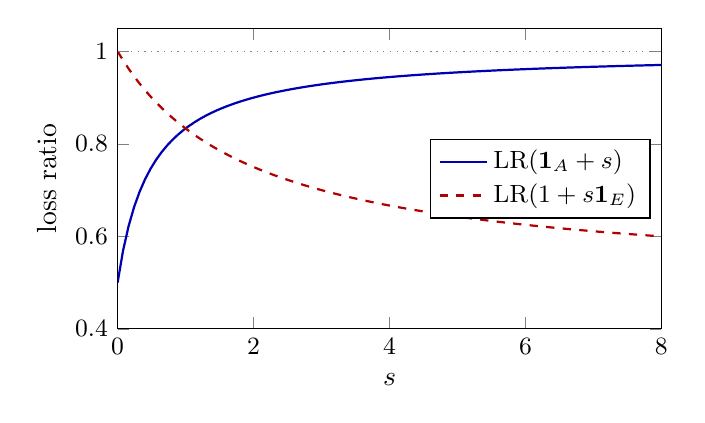
\begin{tikzpicture}
\begin{axis}[width=0.7\textwidth,height=5.4cm,xmin=0,xmax=8,ymin=0.4,ymax=1.05,
  xlabel={$s$},ylabel={loss ratio},tick label style={font=\small},samples=100,domain=0:8,
  legend style={font=\small,at={(0.98,0.5)},anchor=east,cells={anchor=west}}]
\addplot[thick,blue!70!black] {(0.25+x)/(0.5+x)};
\addlegendentry{$\LR(\1_A+s)$}
\addplot[thick,red!70!black,dashed] {(1+0.25*x)/(1+0.5*x)};
\addlegendentry{$\LR(1+s\1_E)$}
\addplot[gray,dotted,domain=0:8] {1};
\end{axis}
\end{tikzpicture}
\caption{Example~\ref{ex:F2}: $h=\mathrm{id}$, $g=\sqrt{\cdot}$, $P(A)=P(E)=\frac14$. Both families of books
increase with $s$; the loss ratio increases along one and decreases along the other.}\label{fig:F2}
\end{figure}

\section{Dropping law invariance}\label{supp:A0}

We state the version without \axLI, which covers scenario-dependent loss ratios. A \emph{game} is a map $\nu:\mathcal F\to\R$ with $\nu(\emptyset)=0$. It is
\emph{null-invariant} if $P(A\triangle B)=0$ implies $\nu(A)=\nu(B)$; its \emph{chain variation} is
$\|\nu\|_{bv}=\sup\sum_j|\nu(A_j)-\nu(A_{j-1})|$ over chains
$\emptyset=A_0\subset\dots\subset A_n=\Omega$. Let $\mathcal V_1$ be the null-invariant games with
$\|\nu\|_{bv}<\infty$ and $\nu(\Omega)=1$, and for $\nu\in\mathcal V_1$ let
$C_\nu(X)=\int_0^\infty\nu(X>x)\,dx+\int_{-\infty}^0[\nu(X>x)-1]\,dx$. A \emph{capacity} is a monotone game.

\begin{theorem}[Without law invariance]\label{thm:A0}
$\LR$ satisfies \axPe, \axR{} and \axRC{} if and only if $\LR=C_{\nu_1}/C_{\nu_2}$ where
$C_{\nu_2}\ne0$ and $\LR\notin\R$ where $C_{\nu_2}=0$, for $\nu_1,\nu_2\in\mathcal V_1$; with \axRM{} in place
of \axRC{}, if and only if the same holds with capacities $\nu_1,\nu_2$. The pair is unique:
$\nu_1(A)=\rho(\1_A)$ and $\nu_2(A)=\Pi(\1_A)$. The loss ratio is in addition law invariant if and only if
$\nu_i=k_i\circ P$ with $k_i\in\Hset_1$, which recovers Theorems~\ref{thm:A} and~\ref{thm:B}.
\end{theorem}

The set-function representation in Theorem~\ref{thm:A0} is that of \citet{msm1994} and
\citet{cmmm2012,cmmm2015}; the proof is in Section~\ref{app:A0}.
\subsection{Proof of Theorem~\ref{thm:A0}}\label{app:A0}


Lemmas~\ref{lem:premium}, \ref{lem:implied}, \ref{lem:comon} and~\ref{lem:cashlip} do not use \axLI. Put
$\nu_1(A):=\rho(\1_A)$ and $\nu_2(A):=\Pi(\1_A)$. They are null-invariant, because $\rho$ and $\Pi$ act on
almost-sure classes, normalized by $\rho(1)=\Pi(1)=1$, and the layer formula \eqref{eq:layer} holds with
$\nu_i(C_j)$ in place of $h(P(C_j))$, for every chain $C_1\supset\dots\supset C_m$.

\emph{Bounded variation.} Given a chain $\emptyset=A_0\subset\dots\subset A_n=\Omega$, run the proof of
Lemma~\ref{lem:bv} with $I_j:=A_j\setminus A_{j-1}$; then $\{W\ge2(n-j)\}=A_j$, and one obtains
$\|\nu_1\|_{bv}\le2L$. Under \axRM, $\nu_1$ is monotone, i.e.\ a capacity.

\emph{Jordan decomposition of a game.} For $\nu\in\mathcal V$ let $\nu^+(A):=\sup\sum_j(\nu(A_j)-\nu(A_{j-1}))^+$
over chains from $\emptyset$ to $A$, and $\nu^-:=\nu^+-\nu$.
For $A\subset B$, appending $B$ to a chain for $A$ gives $\nu^+(B)\ge\nu^+(A)+(\nu(B)-\nu(A))^+$. Hence $\nu^+$ is
non-decreasing, and $\nu^-(B)-\nu^-(A)\ge(\nu(B)-\nu(A))^+-(\nu(B)-\nu(A))\ge0$, so $\nu^-$ is non-decreasing.
Moreover $\nu^+(A)\le\|\nu\|_{bv}$ (append $\Omega$), and null-invariance passes to $\nu^\pm$ (if $P(A\triangle A')=0$,
map $A_j\mapsto A_j\cap A'$ for $j<n$ and $A_n\mapsto A'$, which preserves all $\nu$-values).

\emph{Representation.} $C_{\nu^\pm}$ (with the correction term by $\nu^\pm(\Omega)$) is monotone with cash slope
$\nu^\pm(\Omega)$, hence Lipschitz, and $C_\nu=C_{\nu^+}-C_{\nu^-}$ by linearity in $\nu$. Now $\rho$ and
$C_{\nu_1}$ are Lipschitz and agree on simple positions by \eqref{eq:layer}, so $\rho=C_{\nu_1}$; likewise
$\Pi=C_{\nu_2}$.

\emph{Converse and uniqueness.} As in the proof of Theorems~\ref{thm:A} and~\ref{thm:B}, with $\nu$ in place of
$h\circ P$; null-invariance makes $C_\nu$ well defined on almost-sure classes and makes almost-sure nestedness
sufficient. Uniqueness follows because $\Pi(\1_A)$ is minus the price point of $\1_A$ and $\rho(\1_A)$ is given by
Proposition~\ref{prop:readings}(b).

\emph{Law invariance.} If \axLI{} holds, Lemma~\ref{lem:LI} makes $\nu_i(A)$ a function of $P(A)$ alone, so
$\nu_i=k_i\circ P$; since the space is atomless, $\|k\circ P\|_{bv}=\TV(k)$, so $k_i\in\Hset_1$. Conversely
$k\circ P$ gives a law-invariant functional. \qed


\section{Nonnegative losses}\label{sec:actuarial}

Insurance losses are nonnegative and premiums are positive. On $\Xp=L^\infty_+\setminus\{0\}$ only upward
shifts $X+c$, $c\ge0$, are available, and the price point $-\Pi(X)<0$ lies outside the domain, so that \axP{}
cannot be used; nor can \axPe{} and \axR, which pool books after moving them to zero premium. The axioms
of this section are therefore stated with reals attached to the cash lines; restating them in terms of values of
$\LR_0$ alone, as in Section~\ref{sec:axioms}, is left open. In this section the loss ratio is a map $\LR_0:\Xp\to\R$, and $N_0:=\{X\in\Xp:\LR_0(X)=1\}$.

\subsection{Axioms}

\begin{definition}[Axioms (A0)--(A5)]\label{def:Axioms}
\begin{description}[leftmargin=0pt,labelindent=0pt,itemsep=3pt,style=unboxed]
\item[(A0)] $N_0$ has empty interior in $(\Xp,\|\cdot\|_\infty)$.
\item[(A1)] For each $X\in\Xp\setminus N_0$ there are reals $a_X,b_X$ with $\LR_0(X+c)=(a_X+c)/(b_X+c)$ for all
  $c\ge0$. By Lemma~\ref{lem:halfline}, $a_X\ne b_X$, the pair is unique and $b_X>0$; put $\rho(X):=a_X$ and
  $\Pi(X):=b_X$ on $\Xp\setminus N_0$.
\item[(A2)] $\LR_0$ is law invariant.
\item[(A3)] $\rho$ and $\Pi$ are non-decreasing on $\Xp\setminus N_0$. Variant (A3$_s$): $\rho$ and $\Pi$ are
  uniformly continuous on $\Xp\setminus N_0$.
\item[(A4)] Let $\bar\rho,\bar\Pi$ be the continuous extensions of $\rho,\Pi$ to $\Xp$ (they exist under (A3) or
  (A3$_s$) by Lemma~\ref{lem:ext}). For comonotone $X,Y\in\Xp$:
  \begin{itemize}[nosep]
  \item[(A4a)] $\bar\Pi(X+Y)=\bar\Pi(X)+\bar\Pi(Y)$;
  \item[(A4b)] $\bar\Pi(X+Y)\LR_0(X+Y)=\bar\Pi(X)\LR_0(X)+\bar\Pi(Y)\LR_0(Y)$.
  \end{itemize}
\item[(A5)] $\LR_0$ is norm-continuous on $\Xp$.
\end{description}
\end{definition}

Axiom (A0) excludes $\LR_0\equiv1$, for which $\rho$ and $\Pi$ are not identified, and ensures that $\rho,\Pi$ are
defined on a dense set. Axiom (A1) is the counterpart of Proposition~\ref{prop:readings}(a) on a half line: since
the price point is not observed, the premium must be extrapolated from $c\ge0$, which requires the functional
form to be assumed rather than derived. Axiom (A4b) is the pooling identity \axCM, and (A4a) states that premiums
add under comonotone pooling; on $\Xp$ the two must be stated separately. Axiom (A5) excludes jumps of $\LR_0$
where the premium distortion vanishes; it excludes, for example, value-at-risk-type premium distortions
$g=\1_{(a,1]}$, and it implies $g>0$ (Step C5 in Appendix~\ref{app:C}).

\begin{lemma}\label{lem:halfline}
If $X\notin N_0$ satisfies (A1) with $(a,b)$, then $a\ne b$, the pair is unique, $b>0$, and for every
$c_0\ge0$ one has $X+c_0\notin N_0$ with $\rho(X+c_0)=\rho(X)+c_0$ and $\Pi(X+c_0)=\Pi(X)+c_0$.
\end{lemma}

\subsection{Results}

\begin{theorem}\label{thm:C}
$\LR_0$ satisfies (A0)--(A5) if and only if $\LR_0=C_h/C_g$ on $\Xp$ for distortion functions $h\ne g$
with $g>0$ on $(0,1]$. In that case $(h,g)$ is unique, also among pairs in $\Hset_1^2$ with
$C_{g'}>0$ on $\Xp$; moreover $\bar\rho=C_h$, $\bar\Pi=C_g$ and $N_0=\Xp\cap\{C_h=C_g\}$.
\end{theorem}

\begin{theorem}\label{thm:Cp}
Axioms (A0)--(A2), (A3$_s$), (A4) and (A5) hold if and only if $\LR_0=C_h/C_g$ with $h,g\in\Hset_1$, $h\ne g$,
and $g>0$ on $(0,1]$.
\end{theorem}

\begin{proposition}\label{prop:bridge}
$\LR_0=C_h/C_g$ with distortion functions $h,g$ and $g>0$ on $(0,1]$ if and only if $\LR_0$ is the restriction to
$\Xp$ of an extended loss ratio satisfying the axioms of Theorem~\ref{thm:B} with $\Pi>0$ on $\Xp$. The representing
pair $(h,g)$ of such an extension is unique if and only if $\LR_0\not\equiv1$. In that case the extension is unique up
to the labels $\infty,\star$ at its non-finite values, and unique under convention \ax{S}.
\end{proposition}

Theorem~\ref{thm:C} is the loss-ratio analogue of the characterization of \citet{wyp1997}. Unlike that result,
the pair $(\rho,\Pi)$ is defined only off $N_0$, and positivity of $g$ is derived from (A5). The proofs are given in
Appendix~\ref{app:C}, and Section~\ref{sec:necessity} shows that none of (A2)--(A5) can be dropped.

\subsection{Witnesses for the actuarial axioms}\label{supp:actwit}

\begin{table}[ht]
\centering\small
\begin{tabularx}{\textwidth}{@{}l>{\raggedright\arraybackslash}p{4.6cm}>{\raggedright\arraybackslash}X@{}}
\toprule
\textbf{Dropped} & \textbf{Witness on $\Xp$} & \textbf{Reason}\\
\midrule
(A2) & $\E_Q/\E$ & $N_0$ lies in a closed hyperplane, so (A0) holds; not law invariant.\\
(A3) & $C_h/\E$, $h=t+\tfrac14\sin2\pi t$ & $\rho(\1_A)>\rho(\1_B)$ for $\1_A\le\1_B$, $P(A)=0.4,P(B)=0.6$.\\
(A3$_s$) & $C_h/\E$, $h$ continuous non-BV & Extensions exist; $h$ is not of bounded variation.\\
(A4a) & $\E/\max(C_{\sqrt t},C_{\min(1,1.5t)})$ & Premium is not comonotonic additive (numbers above); (A4b) holds.\\
(A4b) & $\max(C_{\sqrt t},C_{\min(1,1.5t)})/\E$ & $\bar\Pi=\E$ additive, but $\bar\Pi\LR_0$ is not.\\
(A5) & $C_h/C_g$ with $g=(2t-1)^+$, $h=g^2$, and $\LR_0:=1$ where $C_g=0$ & $\LR_0$ jumps: $\LR_0(\1_B+n^{-1}\1_C)=\tfrac12$ while $\LR_0(\1_B)=1$ for $P(B)\le\tfrac12$, $C\supset B$, $P(C)=\tfrac34$.\\
\bottomrule
\end{tabularx}
\caption{Witnesses for (A2)--(A5) on the actuarial domain. In each case all other axioms hold.}\label{ex:A5}
\end{table}
\subsection{Proofs}\label{app:C}


\begin{proof}[Proof of Lemma~\ref{lem:halfline}]
$a/b=\LR_0(X)\ne1$, so $a\ne b$. \emph{Uniqueness.} If $(a+c)(b'+c)=(a'+c)(b+c)$ for all $c\ge0$, comparing
coefficients gives $a+b'=a'+b$ and $ab'=a'b$; writing $a'=a+t$, $b'=b+t$ gives $t(a-b)=0$, so $t=0$.
\emph{Positivity.} If $b\le0$, the pole $-b\ge0$, at which the numerator does not vanish, would contradict finiteness
of $\LR_0$. \emph{Shifts.} $\LR_0(X+c_0)=(a+c_0)/(b+c_0)\ne1$, and the profile of $X+c_0$ is the shifted profile of $X$. \qedhere
\end{proof}

\begin{lemma}[Sierpi\'nski and quantile coupling]\label{lem:coupling}
(a) If $P(B)>0$, $P(\cdot\mid B)$ carries a uniform random variable. (b) For every $Y\in L^\infty$ there is a uniform
$U$ with $Y=q_Y(U)$ a.s. If $X\eqd Y$ and $X_n\to X$ in norm, then $Y_n:=q_{X_n}(U)$ satisfies $Y_n\eqd X_n$ and
$\|Y_n-Y\|\le\|X_n-X\|$.
\end{lemma}

\begin{proof}
(a) $P(\cdot\mid B)$ is atomless; by Sierpi\'nski's theorem there are sets $B_t\subset B$, increasing in dyadic
$t\in[0,1]$, with $B_1=B$ and $P(B_t)=tP(B)$. Put $W:=\inf\{t:\omega\in B_t\}$; then $\{W<t\}\subset B_t\subset\{W\le t\}$,
so $P(W\le t\mid B)=t$. (b) Off the atoms of $Y$ set $U:=F_Y(Y)$; on each atom $\{Y=y\}$ set
$U:=F_Y(y-)+(F_Y(y)-F_Y(y-))W_y$ with $W_y$ uniform under $P(\cdot\mid Y=y)$ by (a). Then $U$ is uniform and
$q_Y(U)=Y$. If $|X_n-X|\le\varepsilon$ a.s., quantiles move by at most $\varepsilon$, so
$\|q_{X_n}(U)-q_X(U)\|\le\|X_n-X\|$ and $q_X=q_Y$. \qedhere
\end{proof}

\begin{lemma}[Extension]\label{lem:ext}
Assume (A0)--(A2) and (A3) (respectively (A3$_s$)). Then $\rho,\Pi$ are $1$-Lipschitz (respectively uniformly
continuous) on $\Xp\setminus N_0$, hence extend uniquely to continuous $\bar\rho,\bar\Pi$ on $\Xp$. The extensions
are cash additive for $c\ge0$, law invariant, monotone under (A3), and $\bar\Pi\ge0$.
\end{lemma}

\begin{proof}
Let $X,Y\notin N_0$ and $t=\|X-Y\|$. Then $Y+t\notin N_0$ (Lemma~\ref{lem:halfline}) and $X\le Y+t$, so (A3) gives
$\rho(X)\le\rho(Y)+t$; thus $\rho,\Pi$ are $1$-Lipschitz, and $\Xp\setminus N_0$ is dense by (A0). Cash additivity
passes to the limit. Monotonicity: if $X\le Y$, choose $X_n,Y_n\notin N_0$ within $1/n$ of $X,Y$; then
$X_n\le Y_n+2/n\notin N_0$, and let $n\to\infty$. Law invariance: $N_0$ is law invariant by (A2), and off $N_0$ so are
$\rho,\Pi$ by uniqueness in Lemma~\ref{lem:halfline}. If $X\eqd Y$ and $X_n\to X$ with $X_n\notin N_0$, then
$Y_n:=q_{X_n}(U)\notin N_0$ satisfies $\rho(Y_n)=\rho(X_n)$ and $Y_n\to Y$ (Lemma~\ref{lem:coupling}), so
$\bar\rho(X)=\bar\rho(Y)$. Finally $\Pi>0$ off $N_0$ gives $\bar\Pi\ge0$. Under (A3$_s$) the same argument applies with
extension by uniform continuity. \qedhere
\end{proof}

\begin{lemma}[Sweep]\label{lem:sweep}
Let $k$ be bounded Borel with $k(0)=0$, such that $C_k$ is comonotonic additive on $\Xp$ (true for $k\in\Hset$ and
for continuous $k$). If $k(p_0)\ne0$ for some $p_0\in(0,1]$, then $\Xp\cap\{C_k=0\}$ has empty interior.
\end{lemma}

\begin{proof}
Write $X=q_X(U)$ and $A=\{U>1-p_0\}$. Then $X$ and $\1_A$ are comonotone, so $C_k(X+t\1_A)=C_k(X)+t\,k(p_0)$ for
$t>0$, which vanishes for at most one $t$. Since $\|X+t\1_A-X\|=t$, every ball around $X$ meets $\{C_k\ne0\}$. \qedhere
\end{proof}

\begin{proof}[Proof of Theorem~\ref{thm:C}]
\emph{Step C1 (law invariance, extension).} Lemma~\ref{lem:ext}.

\emph{Step C2 (pole).} $\bar\Pi$ is comonotonic additive by (A4a) and continuous, hence positively homogeneous. Then
$\bar\Pi(2)=2\bar\Pi(1)$ and $\bar\Pi(2)=\bar\Pi(1)+1$ give $\bar\Pi(1)=1$.

\emph{Step C3 (zero).} $\bar\rho$ and $\LR_0\bar\Pi$ are continuous (by (A5) for the second) and agree off $N_0$,
where $a_X=\LR_0(X)b_X$; so $\bar\rho=\LR_0\bar\Pi$ on $\Xp$. By (A4b), $\bar\rho$ is comonotonic additive, hence
homogeneous, and $\bar\rho(1)=1$ as in C2.

\emph{Step C4 (representation).} For $P(A)=p>0$ put $h(p):=\bar\rho(\1_A)$, $g(p):=\bar\Pi(\1_A)$ and
$h(0)=g(0)=0$. They are well defined (law invariance) and non-decreasing (monotonicity). Since
$\varepsilon\1_A\le\1_A$, homogeneity and monotonicity give $(1-\varepsilon)h(p)\ge0$, so $h,g\ge0$; thus $h,g$ are
distortion functions. A simple $X\in\Xp$ equals $\sum_i(x_i-x_{i-1})\1_{B_i}$ with $x_{-1}=0$, $B_i=\{X\ge x_i\}$,
a comonotone sum of positive multiples of indicators, so $\bar\rho(X)=C_h(X)$; approximating $X$ by the simple
$\lceil nX\rceil/n\in\Xp$ gives $\bar\rho=C_h$ on $\Xp$, and likewise $\bar\Pi=C_g$.

\emph{Step C5 (positivity of $g$).} (a) If $g(p)=0$ then $h(p)=\LR_0(\1_A)\cdot0=0$. (b) By (A0) some $W\notin N_0$
exists and, by Lemma~\ref{lem:halfline}, $\bar\rho(W)\ne\bar\Pi(W)$, so $h(q_0)\ne g(q_0)$ for some $q_0$; as
$g(q_0)\ge0$ and $g(q_0)\ne0$ by (a), $g(q_0)>0$. (c) Suppose $g(p)=0$ for some $p>0$ and take nested $B,C$ with
$P(B)=p$, $P(C)=q_0$ and $X_n=\1_B+n^{-1}\1_C$. Then $\bar\Pi(X_n)=g(q_0)/n>0$, $\bar\rho(X_n)=h(q_0)/n$, so
$\LR_0(X_n)=h(q_0)/g(q_0)\ne1$. But $\bar\Pi(\1_B)=g(p)=0$ forces $\1_B\in N_0$, so $\LR_0(\1_B)=1$, contradicting (A5)
since $X_n\to\1_B$.

\emph{Step C6 (conclusion).} $\LR_0=\bar\rho/\bar\Pi=C_h/C_g$. If $h=g$ then $N_0=\Xp$, contradicting (A0).

\emph{Converse.} Let $\LR_0=C_h/C_g$ with $h\ne g$ and $g>0$ on $(0,1]$; then $C_g>0$ on $\Xp$, because
$P(X>x)>0$ for $x\in[0,\ess X)$. (A1) holds with $a_X=C_h(X)$, $b_X=C_g(X)$;
(A2)--(A5) are immediate; (A0) follows from Lemma~\ref{lem:sweep} with $k=h-g$, since
$N_0=\Xp\cap\{C_{h-g}=0\}$.

\emph{Uniqueness among signed pairs.} If also $\LR_0=C_{h'}/C_{g'}$ with $(h',g')\in\Hset_1^2$ and $C_{g'}>0$, then by
Lemma~\ref{lem:halfline} $C_{h'}=\rho$ and $C_{g'}=\Pi$ off $N_0$. The set $N_0$ is determined by $\LR_0$ and has dense
complement (Lemma~\ref{lem:sweep}, $h\ne g$), so by continuity $C_{h'}=\bar\rho=C_h$ and $C_{g'}=C_g$; evaluating at
indicators gives $h'=h$, $g'=g$. \qedhere
\end{proof}

\begin{proof}[Proof of Theorem~\ref{thm:Cp}]
Steps C1, C2 and the extension hold with uniform continuity in place of monotonicity. For $Z\in L^\infty$ and
$M>\|Z\|$ put $\tilde\rho(Z):=\bar\rho(Z+M)-M$, independent of $M$ by cash additivity. Then $\tilde\rho$ is law
invariant, cash additive, uniformly continuous and comonotonic additive (the shifts $Z_i+M$ are comonotone elements
of $\Xp$, and Step C3 with (A4b) applies). Lemmas~\ref{lem:cashlip}--\ref{lem:rep}, applied to $\tilde\rho$ and
likewise to $\tilde\Pi$ (using (A4a)), give $\tilde\rho=I_h$, $\tilde\Pi=I_g$ with $h,g\in\Hset_1$. Step C5 holds
verbatim: in (b) the sign $g\ge0$ comes from $\bar\Pi\ge0$, not from monotonicity, and in (c) nested sets are
comonotone in either direction. The converse uses the Lipschitz bounds for (A3$_s$) and Lemma~\ref{lem:sweep} for
(A0). \qedhere
\end{proof}

\begin{proof}[Proof of Proposition~\ref{prop:bridge}]
($\Rightarrow$) Extend $\LR_0$ to $L^\infty$ by $\bracket{I_h}{I_g}$; this satisfies Theorem~\ref{thm:B}, and
$I_g>0$ on $\Xp$ because $g>0$. ($\Leftarrow$) Theorem~\ref{thm:B} gives distortions $h,g$, and $I_g>0$ on $\Xp$
forces $g>0$ on $(0,1]$ (otherwise $I_g(\1_A)=g(P(A))=0$ for some $A$). \emph{Uniqueness.} If $\LR_0\not\equiv1$ then
$h\ne g$, and two extensions have pairs that agree by the uniqueness in Theorem~\ref{thm:C}. Their finite values,
$I_h/I_g$ on $\{I_g\ne0\}$, and their non-finite locations, $\{I_g=0\}$, therefore coincide; the labels at the
non-finite values are fixed by \ax{S} and are otherwise arbitrary (for instance, the value at $0$ may be $\infty$ or
$\star$). If $\LR_0\equiv1$, $\bracket{I_{\mathrm{id}}}{I_{\mathrm{id}}}$ and $\bracket{I_{\sqrt\cdot}}{I_{\sqrt\cdot}}$ have
different representing pairs: the price point of $\1_A$ is $-P(A)$ for the first and $-\sqrt{P(A)}$ for the second. \qedhere
\end{proof}

\section{Consequences}\label{sec:consequences}

Throughout this section the axioms of Theorem~\ref{thm:A} and the labelling convention \ax{S} hold, $\LR=\bracket{I_h}{I_g}$, and for
$\beta\neq1$ we put
\[
 \rho_\beta:=\frac{\rho-\beta\Pi}{1-\beta},\qquad
 k_\beta:=\frac{h-\beta g}{1-\beta}=g+\frac{h-g}{1-\beta}\in\Hset_1 .
\]

\begin{corollary}[Association]\label{cor:assoc}
\begin{enumerate}[label=(\alph*),nosep]
\item $\rho_\beta=I_{k_\beta}$ is cash additive of slope $1$, and $\rho_\beta(X)=0\iff\LR(X)\in\{\beta,\star\}$.
  Hence $\LR(X)=\beta\iff\rho_\beta(X)=0$ holds exactly off $\{\rho=\Pi=0\}=\{\LR=\star\}$; it fails, for instance, at
  $X=0$ and at $X-\rho(X)$ for every $X\in N$.
\item For $X\notin N$: $\LR(X-m)=\beta\iff m=\rho_\beta(X)$, and then $\Pi(X)-m=(\Pi(X)-\rho(X))/(1-\beta)\ne0$.
\item For $X\in N$: $\LR(X-m)\in\{1,\star\}$ for every $m$.
\item $\rho_\beta$ is $\TV(k_\beta)$-Lipschitz; in Theorem~\ref{thm:B}, $\TV(k_\beta)\le(1+|\beta|)/|1-\beta|$.
\item $\rho_\beta$ is monotone iff $k_\beta$ is non-decreasing. If $h\ne g$, $\rho_\beta$ is \emph{not} monotone for
  all $\beta$ in a punctured neighbourhood of $1$.
\end{enumerate}
\end{corollary}

\begin{proof}
(a) $\rho_\beta(X)=0\iff\rho(X)=\beta\Pi(X)$; if $\Pi(X)\ne0$ this says $\LR(X)=\beta$, and if $\Pi(X)=0$ it says
$\rho(X)=0$, i.e.\ $\LR(X)=\star$. Conversely $\LR(X)=\star$ means $\rho=\Pi=0$. At $X\in N$, $Y=X-\rho(X)$ has
$\rho(Y)=\Pi(Y)=0$, so $\LR(Y)=\star\ne\beta$ while $\rho_\beta(Y)=0$.
(b) $\LR(X-m)=\beta\iff\rho-m=\beta(\Pi-m)\iff m=\rho_\beta(X)$, and
$\Pi-\rho_\beta=(\Pi-\rho)/(1-\beta)\neq0$ off $N$.
(c) On $N$ the cash line equals $1$ away from its price point (Proposition~\ref{prop:readings}(d)).
(d) Lemma~\ref{lem:cashlip} and the Lipschitz bound for $I_{k}$.
(e) $I_{k}$ is monotone iff $k$ is non-decreasing. Since $h-g$ vanishes at $0$ and $1$ and is non-constant, there are
$p<q$ with $(h-g)(p)>(h-g)(q)$ and $p'<q'$ with $(h-g)(p')<(h-g)(q')$. As $\beta\to1$,
$(1-\beta)k_\beta=h-\beta g\to h-g$ uniformly, so for $\beta$ near $1$ both strict inequalities persist for
$k_\beta$, whatever the sign of $1-\beta$. \qedhere
\end{proof}

Part (e) is the counterpart of Proposition~\ref{prop:F2} for the associated family: even when $\rho$ and $\Pi$ are
distortion premia, $\rho_\beta$ is in general a signed Choquet integral.

\begin{example}\label{ex:family}
Let $h=\mathrm{id}$ and $g=\sqrt{\cdot}$. Then $k_\beta(p)=(p-\beta\sqrt p)/(1-\beta)$ and
$k_\beta'(p)=\big(1-\beta/(2\sqrt p)\big)/(1-\beta)$. For $\beta<1$, $k_\beta$ is non-decreasing if and only if
$\beta\le2\sqrt p$ for all $p\in(0,1]$, that is, $\beta\le0$; for $\beta>1$ it is non-decreasing if and only if
$\beta\ge2\sqrt p$ for all $p$, that is, $\beta\ge2$. Hence $\rho_\beta$ is a distortion premium if and only if
$\beta\notin(0,2)$; for $\beta\in(0,1)\cup(1,2)$ it is a signed Choquet integral that is not monotone
(Figure~\ref{fig:family}).
\end{example}

\begin{figure}[ht]
\centering
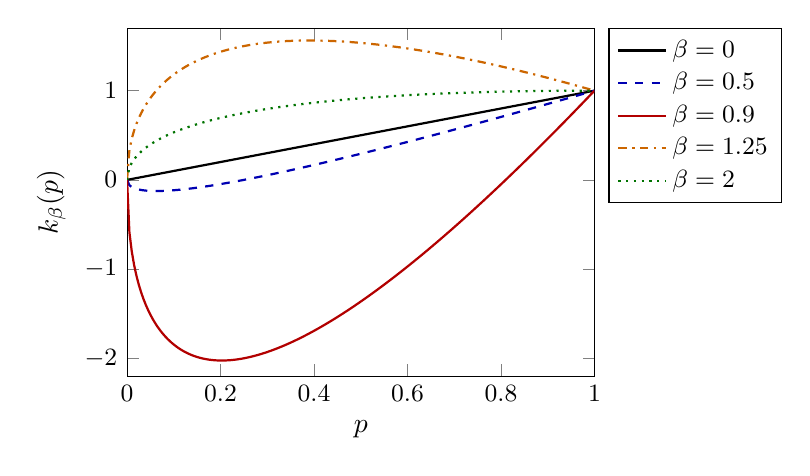
\begin{tikzpicture}
\begin{axis}[width=0.62\textwidth,height=6cm,xmin=0,xmax=1,ymin=-2.2,ymax=1.7,
  xlabel={$p$},ylabel={$k_\beta(p)$},tick label style={font=\small},samples=200,domain=0:1,
  legend pos=outer north east,legend style={font=\small,cells={anchor=west}}]
\addplot[thick,black] {x}; \addlegendentry{$\beta=0$}
\addplot[thick,blue!70!black,dashed] {(x-0.5*sqrt(x))/0.5}; \addlegendentry{$\beta=0.5$}
\addplot[thick,red!70!black] {(x-0.9*sqrt(x))/0.1}; \addlegendentry{$\beta=0.9$}
\addplot[thick,orange!80!black,dashdotted] {(x-1.25*sqrt(x))/(-0.25)}; \addlegendentry{$\beta=1.25$}
\addplot[thick,green!45!black,dotted] {(x-2*sqrt(x))/(-1)}; \addlegendentry{$\beta=2$}
\end{axis}
\end{tikzpicture}
\caption{The distortions $k_\beta$ of the associated family in Example~\ref{ex:family} ($h=\mathrm{id}$,
$g=\sqrt{\cdot}$). They are monotone for $\beta=0$ and $\beta=2$ and not monotone for $\beta\in(0,1)\cup(1,2)$.}
\label{fig:family}
\end{figure}

\begin{corollary}[Pooling at non-finite values]\label{cor:projpool}
Assume the axioms of Theorem~\ref{thm:A} and \ax{S}. Then for all comonotone $X,Y$,
\[
 \LR(X+Y)=\bracket{\rho(X)+\rho(Y)}{\Pi(X)+\Pi(Y)} .
\]
In terms of loss ratios and implied premiums alone:
\begin{center}\small
\begin{tabularx}{0.95\textwidth}{@{}>{\raggedright\arraybackslash}p{5.4cm}>{\raggedright\arraybackslash}X@{}}
\toprule
\textbf{Case} & \textbf{Pooled loss ratio}\\
\midrule
$X,Y\in D$, $\Pi(X)+\Pi(Y)\ne0$ & relative-cost-weighted combination (\axCM)\\
$X,Y\in D$, premiums cancel & $\infty$ if $\LR(X)\ne\LR(Y)$; $\star$ if $\LR(X)=\LR(Y)$\\
$\Pi(X)=0$, $Y\in D$ & $\LR(Y)+\rho(X)/\Pi(Y)$, with $\rho(X)=\lim_{c\to0}c\,\LR(X+c)$\\
$\Pi(X)=\Pi(Y)=0$ & $\infty$ unless $\rho(X)=-\rho(Y)$, in which case $\star$\\
\bottomrule
\end{tabularx}
\end{center}
\end{corollary}

\begin{proof}
$\rho$ and $\Pi$ are comonotonic additive (Lemma~\ref{lem:comon}) and $\LR=\bracket{\rho}{\Pi}$ under \ax{S}
(Theorem~\ref{thm:A}). The table spells out $\bracket{\rho(X)+\rho(Y)}{\Pi(X)+\Pi(Y)}$, using $\rho=\Pi\,\LR$ on $D$
and Proposition~\ref{prop:readings}(c) for books with zero premium. If premiums cancel,
$\rho(X)+\rho(Y)=\Pi(X)(\LR(X)-\LR(Y))$. \qedhere
\end{proof}

The third row has a direct reading: a loss that is carried without premium adds its size, relative to the
premium base, to the loss ratio of the book it joins.

\begin{corollary}[Orderings, convexity and shape within the class]\label{cor:shape}
\begin{enumerate}[label=(\alph*)]
\item \emph{Endpoints.} $\rho$ is monotone iff $h$ is non-decreasing; $\rho$ is convex iff $h$ is concave
  \citep[Thm.~3]{www2020}; $\rho$ is coherent iff $h$ is concave and non-decreasing, in which case $\rho$ is a
  mixture of expected shortfalls $\mathrm{ES}_\alpha$ over levels $\alpha\in[0,1]$, with the convention
  $\mathrm{ES}_1:=\operatorname{ess\,sup}$ \citep{kusuoka2001,jst2006,folmerschied2016} and \citet[Thm.~5]{www2020b}; the endpoint is needed, for
  instance, for $h=\1_{(0,1]}$, which gives $\rho=\operatorname{ess\,sup}$. The same holds for $\Pi$ and $g$.
\item \emph{Ordering.} $\LR\le1$ on $\{\Pi>0\}$ iff $h\le g$.
\item \emph{Convex acceptance cones.} For $\beta\ne1$ let $A_\beta:=\{\rho\le\beta\Pi\}=\{I_{h-\beta g}\le0\}$.
  Then $A_\beta$ is convex iff $h-\beta g$ is concave, and all $A_\beta$, $\beta\in[0,\infty)\setminus\{1\}$, are
  convex iff $h$ is concave and $g$ is convex.
\item \emph{Quasi-convexity and quasi-concavity (sufficient conditions).}
  If $h$ is concave and $g$ is convex, then $\{\Pi>0\}$ is convex, $\LR\ge1$ there, and $\LR$ is quasi-convex on it.
  If, in Theorem~\ref{thm:B} with $g>0$, $h$ is convex and $g$ is concave, then $\LR\le1$ on $\Xp$ and $\LR$ is
  quasi-concave on $\Xp$. In particular the actuarial ratio $\E/C_g$ with $g$ concave is quasi-\emph{concave}.
\item \emph{Rigidity.} $\rho_\beta$ is convex for all $\beta\in[0,\infty)\setminus\{1\}$ iff $h=g$ and $g$ is concave.
\end{enumerate}
\end{corollary}

\begin{proof}
(a) The monotonicity criterion is in \citet{www2020}, see also \citet[Prop.~2]{www2020b}, and the
convexity criterion is \citet[Thm.~3]{www2020}.
(b) If $h\le g$ then $g-h\ge0$ with $(g-h)(1)=0$, so $I_{g-h}\ge0$ and $\LR\le1$ where $\Pi>0$. If $h(p)>g(p)$ for some $p$,
then $\LR(\1_A+c)=(h(p)+c)/(g(p)+c)>1$ for large $c$, where the premium $g(p)+c$ is positive.
(c) $I_{h-\beta g}$ has cash slope $1-\beta\ne0$, so all its sublevel sets are translates of $A_\beta$; hence
convexity of $A_\beta$ is quasi-convexity of $I_{h-\beta g}$, which is equivalent to concavity of $h-\beta g$
\citep[Thm.~3]{www2020}. Taking $\beta=0$ and $\beta\to\infty$ in $(h-\beta g)/\beta$ gives the second statement.
(d) If $h$ is concave and $g$ is convex then $I_g$ is concave, so $\{I_g>0\}$ is convex; $h\ge\mathrm{id}\ge g$, so
$\LR\ge1$; and for $\beta\ge1$ the set $\{I_h-\beta I_g\le0\}$ is convex because $h-\beta g$ is concave. If
$h$ is convex and $g$ concave, then $h\le\mathrm{id}\le g$, and $I_h-tI_g$ is concave for $t\ge0$, so
$\{\LR\ge t\}$ is convex; for $t<0$ the superlevel set is all of $\Xp$, since $I_h\ge0$ and $I_g>0$ on $\Xp$.
(e) Convexity of $\rho_\beta=I_{k_\beta}$ for $\beta<1$ means $h-\beta g$ concave, and for $\beta>1$ means
$h-\beta g$ convex. Letting $\beta\to1^\mp$ gives $h-g$ concave and convex, hence affine with zero endpoints, i.e.\
$h=g$; then $k_\beta=g$ and $\rho_\beta$ is convex iff $g$ is concave. The converse is clear. \qedhere
\end{proof}

In particular, the actuarial ratio $\E/C_g$ with $g$ concave is quasi-concave and not, in general, quasi-convex.

\begin{example}\label{ex:qc}
Let $A,B$ be disjoint with $P(A)=0.2$, $P(B)=0.3$, and $X_t=(1-t)\1_A+t\1_B$, $t\in[0,1]$. For
$\mathrm{ES}_{0.9}/\E$ (Example~\ref{ex:ES}), $\mathrm{ES}_{0.9}(X_t)=\max\{1-t,t\}$ and
$\LR(X_t)=\max\{1-t,t\}/(0.2+0.1t)$, which equals $5$ at $t=0$, $10/3$ at $t=1$ and $2$ at $t=\tfrac12$: the ratio
lies below the larger endpoint value, as quasi-convexity requires. For $\E/C_{\sqrt{\cdot}}$ the ratio equals
$\sqrt{0.2}\approx0.447$ at $t=0$, $\sqrt{0.3}\approx0.548$ at $t=1$ and $\sqrt{0.5}\approx0.707$ at $t=\tfrac12$: it lies
above the smaller endpoint value, as quasi-concavity requires (Figure~\ref{fig:qc}).
\end{example}

\begin{figure}[ht]
\centering
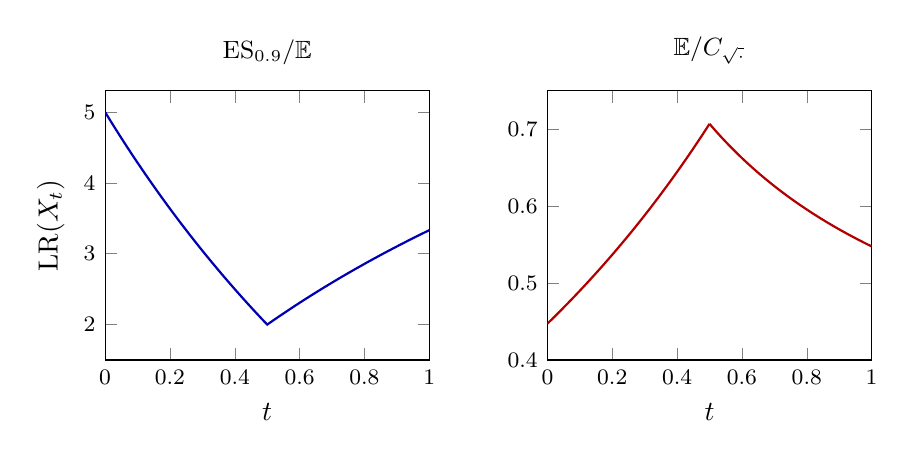
\begin{tikzpicture}
\begin{axis}[name=l,width=0.47\textwidth,height=5cm,xmin=0,xmax=1,ymin=1.5,ymax=5.3,xlabel={$t$},
  ylabel={$\LR(X_t)$},title={\small $\mathrm{ES}_{0.9}/\E$},tick label style={font=\footnotesize},samples=101,domain=0:1]
\addplot[thick,blue!70!black] {max(1-x,x)/(0.2+0.1*x)};
\end{axis}
\begin{axis}[at={(l.south east)},xshift=1.5cm,width=0.47\textwidth,height=5cm,xmin=0,xmax=1,ymin=0.4,ymax=0.75,
  xlabel={$t$},title={\small $\E/C_{\sqrt{\cdot}}$},tick label style={font=\footnotesize},samples=60]
\addplot[thick,red!70!black,domain=0:0.5] {(0.2+0.1*x)/(0.70711*x+0.44721*(1-2*x))};
\addplot[thick,red!70!black,domain=0.5:1] {(0.2+0.1*x)/(0.70711*(1-x)+0.54772*(2*x-1))};
\end{axis}
\end{tikzpicture}
\caption{Loss ratios along the segment $X_t=(1-t)\1_A+t\1_B$ of Example~\ref{ex:qc}: quasi-convex for
$\mathrm{ES}_{0.9}/\E$ (left) and quasi-concave for $\E/C_{\sqrt{\cdot}}$ (right).}\label{fig:qc}
\end{figure}

\begin{example}[Further special cases]
(1) \emph{Wang--Young--Panjer pairs} on nonnegative losses: Theorem~\ref{thm:C}.
(2) \emph{Coherent pairs}: $h,g$ concave non-decreasing; $\rho_\beta$ is a signed mixture of expected shortfalls.
(3) \emph{Actuarial ratio} $\E/C_g$, $h=\mathrm{id}$: Proposition~\ref{prop:unique} gives $g(p)=p/\LR(\1_A)$ for $P(A)=p$, so the
premium distortion is identified from the loss ratios of Bernoulli books.
(4) \emph{VaR-type pairs} are admissible in Theorem~\ref{thm:B}; $\rho_\beta$ is non-monotone near $\beta=1$; a
VaR-type premium $g=\1_{(a,1]}$ is excluded from Theorem~\ref{thm:C}, since $g>0$ fails.
(5) \emph{Gini-type ratios}: $\LR-1=I_{h-g}/I_g$ is a location-invariant signed Choquet ``variability'' divided by a
premium (compare \citealp{bfww2022}).
\end{example}

\section{Positioning in the literature}\label{sec:lit-table}

Table~\ref{tab:littable} summarizes how the case-study result relates to the literatures reviewed in Section~\ref{sec:lit} of the paper.


\begin{table}[ht]
\centering\small
\begin{tabularx}{\textwidth}{@{}>{\raggedright\arraybackslash}p{3.1cm}>{\raggedright\arraybackslash}X>{\raggedright\arraybackslash}X@{}}
\toprule
\textbf{Literature} & \textbf{What it characterizes} & \textbf{Difference from this paper}\\
\midrule
Yaari (1987); Wang, Young, Panjer (1997)
 & One premium functional $H$; axioms on $H$ (law invariance, monotonicity, comonotonic additivity).
 & We characterize a \emph{ratio} of two such functionals with axioms on the ratio. Monotonicity is placed on the \emph{implied premium and risk measure}, never on the ratio.\\
Schmeidler (1986); Murofushi--Sugeno--Machida (1994); Cerreia-Vioglio et al.\ (2012, 2015); Wang--Wei--Willmot (2020)
 & Representation of one comonotonic additive functional as a (signed) Choquet integral.
 & Used as the engine (applied to $\rho$ and $\Pi$). New: the axioms are on $\LR$, comonotonic additivity of $\rho$ and $\Pi$ is \emph{derived} (also on the break-even set), and uniqueness is unconditional.\\
Cherny--Madan (2009); Bielecki--Cialenco--Zhang (2014); Biagini--Bion-Nadal (2014)
 & Monotone, quasi-concave indices $\Leftrightarrow$ increasing families of coherent measures.
 & $\LR$ cannot be monotone (Prop.~\ref{prop:F2}); the associated family is signed and non-monotone. Cardinal (pooling identity) rather than ordinal.\\
Cheridito--Kromer (2013)
 & Axioms for reward--risk ratios (sufficient conditions).
 & Reward over risk is monotone; loss over premium is not. We give an \emph{iff}, within a stated class.\\
Han--Lin--Wang (2025)
 & Diversification quotient: iff axiomatization of a level-crossing index.
 & Closest in spirit; monotone families and a portfolio index. We characterize the ratio and its parts.\\
Haezendonck--Goovaerts (1982); Li--Wang (2023); Bellini et al.\ (2018)
 & Implicitly defined premia/risk measures, return risk measures.
 & Existence and uniqueness of an implicit functional, not a ratio representation. The association is recovered as a corollary and shown to hold only off $\{\rho=\Pi=0\}$.\\
Chew (1983); Dekel (1986)
 & Ratio (weighted utility) versus implicit (betweenness) representations.
 & Explains why a mediant inequality is not enough and a premium-weighted identity is needed.\\
Gneiting (2011)
 & Elicitability of ratios of expectations.
 & Statistical, no axioms on pooling or cash shifts.\\
\bottomrule
\end{tabularx}
\caption{Positioning of the case-study result. ``Iff'' means a characterization by necessary and sufficient axioms.}\label{tab:littable}
\end{table}
\section{The Lean check: process record}\label{supp:lean}

The Lean file was written by the main assistant. Lean could not be installed in the assistant's cloud workspace,
whose network policy blocks the servers that distribute Lean, so the file was compiled on the author's computer.
The author installed Lean and created the project; the assistant read the build output from the project folder
through the link between the Claude desktop application and the author's computer, wrote corrected versions of the
file into the same folder, and the author ran the next build (Figure~\ref{fig:leanloop}).

\begin{figure}[ht]
\centering
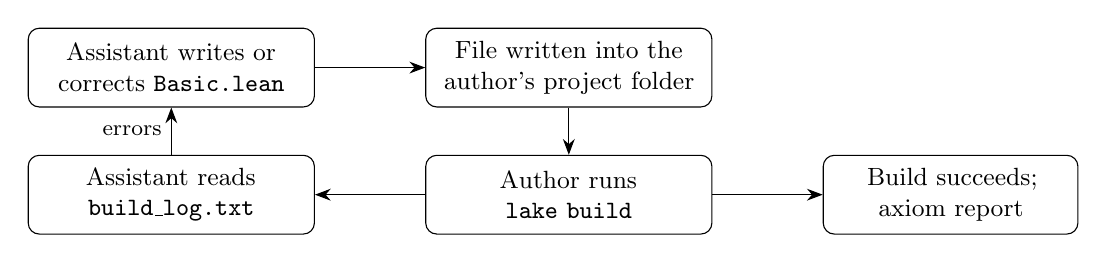
\begin{tikzpicture}[node distance=6mm and 14mm,
  box/.style={draw,rounded corners,align=center,font=\small,minimum height=10mm,text width=34mm},
  >={Stealth[length=2mm]}]
\node[box] (a) {Assistant writes or\\corrects \texttt{Basic.lean}};
\node[box,right=of a] (b) {File written into the\\author's project folder};
\node[box,below=of b] (c) {Author runs\\\texttt{lake build}};
\node[box,left=of c] (d) {Assistant reads\\\texttt{build\_log.txt}};
\draw[->] (a) -- (b);
\draw[->] (b) -- (c);
\draw[->] (c) -- (d);
\draw[->] (d) -- node[left,font=\footnotesize,align=center]{errors}(a);
\node[box,right=of c,text width=30mm] (e) {Build succeeds;\\axiom report};
\draw[->] (c) -- (e);
\end{tikzpicture}
\caption{The build-and-repair loop used for the Lean check.}\label{fig:leanloop}
\end{figure}

Table~\ref{tab:leantime} gives the timeline. Times are in UTC and are taken from the session records and from the
modification times of the files in the project folder.

\begin{table}[ht]
\centering\small
\begin{tabular}{@{}>{\raggedright\arraybackslash}p{3.3cm}>{\raggedright\arraybackslash}p{11.0cm}@{}}
\toprule
\textbf{Time (UTC)} & \textbf{Step}\\
\midrule
21 Oct, 21:38 & The assistant writes a first Lean file for the results in Table~\ref{tab:lean}; it cannot be compiled
  in the cloud workspace.\\
24 Oct, 17:08 & The author asks how a formal proof check can be used; the assistant describes what is feasible
  (the loss-ratio steps), what is hard (the representation step) and how to install Lean.\\
24 Oct, 17:26--17:31 & The author installs the Lean extension for the code editor and the Lean toolchain manager.\\
24 Oct, 17:35--17:37 & The author creates the project \texttt{loss\_ratio\_lean} with Mathlib; Lean and Mathlib
  version~4.36.0-rc1; the precompiled Mathlib files are downloaded.\\
24 Oct, 17:38--17:39 & The assistant inspects the project configuration, confirms that it is complete, and places
  the Lean file in it, replacing the template placeholder.\\
25 Oct, 12:47--12:53 & First attempt to build: the command \texttt{lake} is not found, because the toolchain had not
  been added to the terminal's search path; fixed by loading the toolchain environment.\\
25 Oct, 12:55 & Build 1: four errors, none in a definition or statement. One proof stopped one algebraic step short;
  in three proofs Lean's simplifier rewrote $\mathrm{const}(-c)$ as $-\mathrm{const}(c)$, so that cash additivity
  no longer applied.\\
25 Oct, 12:57 & The assistant writes a corrected file and appends \texttt{\#print axioms} for ten main theorems.\\
25 Oct, 13:04 & Build 2: one error, in the converse construction, where the goal was displayed in an unexpanded
  form. The axiom report shows the three standard axioms for nine theorems and \texttt{sorryAx} for the converse.\\
25 Oct, 13:05 & The assistant adds one line that states the goal explicitly.\\
25 Oct, 13:08 & Build 3 succeeds. All ten theorems depend only on the three standard axioms.\\
25 Oct, 13:09 & The assistant compares the Lean definitions of \axP, \axN, \axCM{} and \axLI{} and the theorem
  statements with Section~\ref{sec:axioms}.\\
25 Oct, 13:37 & At the author's request, the project's own build output is deleted and the file is rebuilt from
  scratch: success in 8.8\,s, with the same axiom report.\\
\bottomrule
\end{tabular}
\caption{Timeline of the Lean check.}\label{tab:leantime}
\end{table}



\bibliography{refs}
\end{document}
